% TikZ shapes: Circle
% Discrete event System
% Latexdraw.com
% 20/01/2021 at 13:55

\documentclass[border=0.2cm]{standalone}

% More defined colors
\usepackage[dvipsnames]{xcolor}

% Required package
\usepackage{tikz}

% Create style for node circles
\tikzstyle{state}=[
	circle,
	minimum size =1.25cm,
	draw=black,
	thick,
	fill=OliveGreen,
	text=white
]

\begin{document}

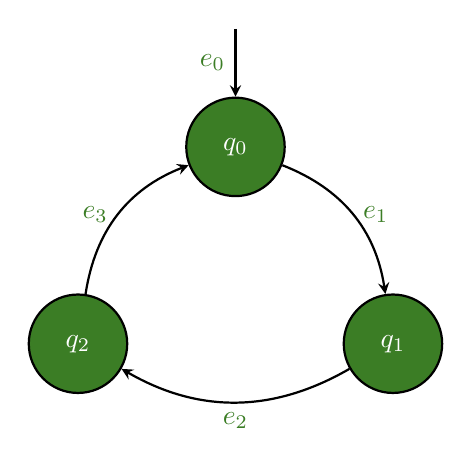
\begin{tikzpicture}[-stealth,thick,text=OliveGreen]

% State q2
\node[state] (A) at (0,0){$q_2$};

% State q1
\node[state] (B) at (4,0){$q_1$};

% State q0
\node[state] (C) at (2,2.5){$q_0$};

% Transition q2 to q0
\draw (A) to[bend left] node[left]{$e_3$}(C) ;

% Transition q0 to q1
\draw (C) to[bend left] node[right]{$e_1$}(B);

% Transition q1 to q2
\draw (B) to[bend left]node[below]{$e_2$} (A);

% Initial state
\draw (2,4) -- node[left]{$e_0$}(C.north);

\end{tikzpicture}

\end{document}
